%% METADATA
%% subject-code: SUBJECT001
%% subject-name: Subject Name
%% semester: 1
%% examination: Sample-2025
%% date: 01-01-2025
%% description: Sample solution guide demonstrating LaTeX conventions for GTU exam solutions
%% summary: Complete example showing proper structure, formatting, and content organization
%% tags: study-material, solutions, sample, gtu, subject001
%% END METADATA

\documentclass{article}

% content/resources/templates/preamble.tex
\usepackage[margin=0.6in]{geometry}
\author{Milav Dabgar}
\usepackage{amsmath,amssymb,amsthm}
\usepackage{booktabs}
\usepackage{multirow}
\usepackage{xcolor}
\usepackage{tcolorbox}
\tcbuselibrary{breakable,skins}
\usepackage[colorlinks=true,linkcolor=blue]{hyperref}
\usepackage{titlesec}
\usepackage{enumitem}
\usepackage{tikz}
\usepackage{pgfplots}
\usepackage{circuitikz}
\usepackage[version=4]{mhchem}
\usepackage{longtable}
\usepackage{array}
\usepackage{float}
\usepackage{caption}
\usepackage{listings}

\lstset{
  basicstyle=\small\ttfamily,
  breaklines=true,
  breakatwhitespace=false,
  postbreak=\mbox{\textcolor{red}{$\hookrightarrow$}\space},
  float=false,
  numbers=left,
  numberstyle=\tiny\color{gray},
  numbersep=10pt,
  xleftmargin=2em,
  keywordstyle=\color{blue},
  commentstyle=\color{green!60!black},
  stringstyle=\color{purple},
  backgroundcolor=\color{gray!5},
  showstringspaces=false,
  tabsize=2,
  captionpos=b,
  keepspaces=true,
  columns=flexible
}

\pgfplotsset{compat=1.18}
\usetikzlibrary{shapes,arrows,positioning,calc,patterns,decorations.pathmorphing,decorations.markings,arrows.meta}

% Color scheme
\definecolor{headcolor}{RGB}{0,102,204}
\definecolor{keycolor}{RGB}{220,20,60}
\definecolor{solutioncolor}{RGB}{34,139,34}
\definecolor{mnemoniccolor}{RGB}{148,0,211}
\definecolor{codecolor}{RGB}{0,0,100}

% Spacing
\setlength{\parskip}{3pt}
\setlist[itemize]{nosep}
\setlist[enumerate]{nosep}

% Title formatting
\titleformat{\section}{\Large\bfseries\color{headcolor}}{\thesection}{1em}{}
\titleformat{\subsection}{\large\bfseries\color{headcolor}}{\thesubsection}{1em}{}

% Pandoc tightlist compatibility
\providecommand{\tightlist}{%
  \setlength{\itemsep}{0pt}\setlength{\parskip}{0pt}}

% Pandoc longtable compatibility
\newcounter{none}
\def\thenone{}


\title{Subject Name (SUBJECT001) - Sample Term Solution}
\date{Month Day, Year}

% PDF Metadata
\hypersetup{
  pdftitle={Subject Name (SUBJECT001) - Sample Term Solution},
  pdfsubject={GTU Exam Solution - Sample-2025},
  pdfauthor={Milav Dabgar},
  pdfkeywords={study-material, solutions, sample, gtu, subject001},
  pdfcreator={XeLaTeX}
}

\begin{document}
\maketitle

\setcounter{tocdepth}{5}
\tableofcontents
\newpage

% ========================================
% QUESTION 1(a): Programming Code (3 marks)
% Demonstrates: lstlisting for code, straight quotes in code, ~100 words
% ========================================

\section{Question 1}

\subsection{Question 1(a) [3 marks]}
\textbf{Write a Java program to find the maximum of three numbers.}

\subsubsection{Solution}
To find the \textbf{maximum} of three numbers, we use \textbf{conditional statements} (if-else) to compare values. The program takes three numbers as input and returns the \emph{largest value} among them.

\paragraph{Java Program:}
\begin{lstlisting}[language=Java,caption={Find Maximum of Three Numbers}]
public class MaxOfThree {
    public static void main(String[] args) {
        int a = 25, b = 40, c = 15;
        int max;
        
        // Compare first two numbers
        if (a > b) {
            max = a;
        } else {
            max = b;
        }
        
        // Compare result with third number
        if (c > max) {
            max = c;
        }
        
        System.out.println("Maximum number is: " + max);
    }
}
\end{lstlisting}

\paragraph{Output:}
\begin{verbatim}
Maximum number is: 40
\end{verbatim}

\paragraph{Key Points:}
\begin{description}
    \item[Logic:] First compare \texttt{a} and \texttt{b}, store larger in \texttt{max}
    \item[Second Comparison:] Compare \texttt{max} with \texttt{c} to get final maximum
    \item[Alternative:] Can use \texttt{Math.max(a, Math.max(b, c))} for concise code
\end{description}

\paragraph{Mnemonic:}
\emph{MAX: Compare in pairs, update Maximum At eXamination}

% ========================================
% QUESTION 1(b): Mathematics Calculation (4 marks)
% Demonstrates: Math equations, step-by-step calculation, inline \texttt{}, ~150 words
% ========================================

\subsection{Question 1(b) [4 marks]}
\textbf{Calculate the cutoff frequency of an RC low-pass filter with \(R = 1.5\,k\Omega\) and \(C = 100\,nF\). Also find the output voltage if input is 10V at cutoff frequency.}

\subsubsection{Solution}

\paragraph{Given Data:}
\begin{itemize}
    \item Resistance: \(R = 1.5\,k\Omega = 1500\,\Omega\)
    \item Capacitance: \(C = 100\,nF = 100 \times 10^{-9}\,F\)
    \item Input Voltage: \(V_{in} = 10\,V\)
\end{itemize}

\paragraph{Step 1: Calculate Cutoff Frequency}
The \textbf{cutoff frequency} formula for RC low-pass filter is:
\[f_c = \frac{1}{2\pi RC}\]

Substituting values:
\[f_c = \frac{1}{2\pi \times 1500 \times 100 \times 10^{-9}}\]
\[f_c = \frac{1}{2\pi \times 1.5 \times 10^{-4}}\]
\[f_c = \frac{1}{9.42 \times 10^{-4}} = 1061.57\,Hz \approx 1.06\,kHz\]

\paragraph{Step 2: Calculate Output Voltage at Cutoff}
At cutoff frequency, output voltage is \textbf{0.707 times} (or \(\frac{1}{\sqrt{2}}\)) the input voltage:
\[V_{out} = 0.707 \times V_{in} = 0.707 \times 10 = 7.07\,V\]

\paragraph{Results:}
\begin{description}
    \item[Cutoff Frequency:] \(f_c = 1.06\,kHz\)
    \item[Output Voltage:] \(V_{out} = 7.07\,V\) at cutoff
    \item[Attenuation:] \(-3\,dB\) at cutoff frequency
    \item[Phase Shift:] \(-45^\circ\) at cutoff frequency
\end{description}

\paragraph{Mnemonic:}
\emph{RC-Formula:} \(f_c = \frac{1}{2\pi RC}\), \(V_{out} = 0.707 \times V_{in}\) at \(f_c\)

% ========================================
% QUESTION 1(c): Comparison Table (7 marks)
% Demonstrates: Comprehensive comparison, tabularx with caption at TOP, ~250 words
% ========================================

\subsection{Question 1(c) [7 marks]}
\textbf{Compare active and passive electronic components with suitable examples.}

\subsubsection{Solution}

Electronic components are classified into \textbf{active} and \textbf{passive} categories based on their ability to control or amplify electrical energy.

\begin{table}[H]
\centering
\caption{Active vs Passive Components Comparison}
\begin{tabularx}{\textwidth}{lXX}
\toprule
\textbf{Characteristic} & \textbf{Active Components} & \textbf{Passive Components} \\
\midrule
Energy Source & Require external power source & Do not require external power \\
Control Ability & Can control/amplify current flow & Cannot amplify, only regulate \\
Directionality & Usually unidirectional & Bidirectional \\
Power Gain & Provide power gain (\(>1\)) & Power gain is always \(\leq 1\) \\
Examples & Transistors (BJT, FET), Diodes (LED, Zener), ICs (Op-Amp, 555), SCR & Resistors, Capacitors, Inductors, Transformers \\
Function & Amplification, switching, oscillation, rectification & Resistance, capacitance, inductance, filtering \\
Linearity & Can be linear or non-linear & Generally linear \\
\bottomrule
\end{tabularx}
\end{table}

\paragraph{Active Components in Detail:}
\begin{description}
    \item[Transistors:] Used for amplification and switching. BJT uses current control, FET uses voltage control.
    \item[Diodes:] Allow current in one direction. LED emits light, Zener regulates voltage.
    \item[ICs:] Integrated circuits like \texttt{555 timer} (oscillator), op-amps (amplifier).
    \item[Power Requirement:] All active components need DC bias/supply to operate.
\end{description}

\paragraph{Passive Components in Detail:}
\begin{description}
    \item[Resistors:] Oppose current flow, dissipate power as heat. Value in \(\Omega\).
    \item[Capacitors:] Store energy in electric field. Value in Farads (F), blocks DC, passes AC.
    \item[Inductors:] Store energy in magnetic field. Value in Henry (H), opposes AC changes.
    \item[Transformers:] Transfer energy between circuits via magnetic coupling.
\end{description}

\subparagraph{Capacitor Types:}
Capacitors include electrolytic (polarized, high capacitance), ceramic (small, stable), and film (precision) types.

\paragraph{Key Distinction:}
The fundamental difference is that active components can \emph{inject power} into a circuit (amplification), while passive components can only \emph{absorb or store} energy, never increase it.

\paragraph{Mnemonic:}
\emph{ACTIVE = Amplify, Control, Transform; PASSIVE = Resist, Store, Filter}

% ========================================
% QUESTION 1(c OR): Alternative Question (7 marks)
% Demonstrates: OR question format, TikZ diagram with gtu styles, lstlisting, ~250 words
% ========================================

\subsection{Question 1(c) OR [7 marks]}
\textbf{Draw and explain the working of a half-wave rectifier circuit with input and output waveforms.}

\subsubsection{Solution}

A \textbf{half-wave rectifier} converts AC voltage to pulsating DC by allowing only one half-cycle (positive or negative) of the input AC waveform to pass through.

\paragraph{Circuit Diagram:}
\begin{figure}[H]
\centering
\begin{circuitikz}[scale=1.2]
    % AC Source
    \draw (0,0) to[sV, l=\(V_{in}\)] (0,2);
    \draw (0,2) to[short] (2,2);
    
    % Diode
    \draw (2,2) to[D*, l=\(D\)] (4,2);
    
    % Load Resistor
    \draw (4,2) to[short] (5,2);
    \draw (5,2) to[R, l=\(R_L\)] (5,0);
    \draw (5,0) to[short] (0,0);
    
    % Output voltage measurement
    \draw (4.5,2) to[short, *-] (4.5,2.5);
    \node at (4.5,2.7) {\(V_{out}\)};
    \draw (4.5,0) to[short, *-] (4.5,-0.5);
    \node[ground] at (4.5,-0.5) {};
\end{circuitikz}
\caption{Half-Wave Rectifier Circuit}
\end{figure}

\paragraph{Working Principle:}
\begin{description}
    \item[Positive Half-Cycle:] When input AC is positive, diode is forward-biased (conducts). Current flows through load resistor \(R_L\), producing output voltage.
    \item[Negative Half-Cycle:] When input AC is negative, diode is reverse-biased (blocks). No current flows, output voltage is zero.
    \item[Result:] Only positive half-cycles appear at output, creating pulsating DC.
\end{description}

\paragraph{Waveform Representation:}
\begin{figure}[H]
\centering
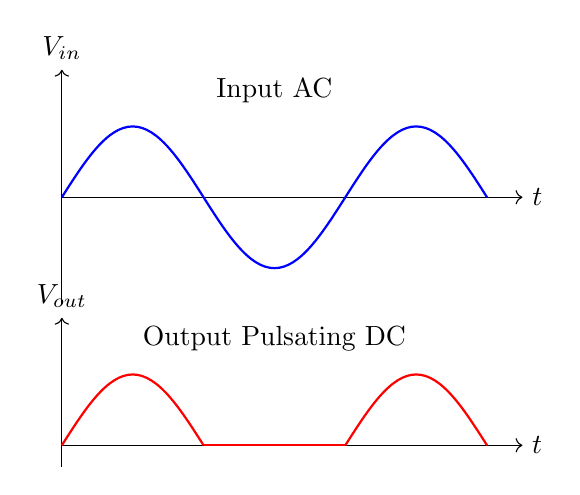
\begin{tikzpicture}[scale=0.9]
    % Input waveform
    \draw[->] (0,0) -- (6.5,0) node[right] {\(t\)};
    \draw[->] (0,-1.5) -- (0,1.8) node[above] {\(V_{in}\)};
    \draw[thick, blue] (0,0) sin (1,1) cos (2,0) sin (3,-1) cos (4,0) sin (5,1) cos (6,0);
    \node at (3,1.5) {Input AC};
    
    % Output waveform
    \begin{scope}[yshift=-3.5cm]
        \draw[->] (0,0) -- (6.5,0) node[right] {\(t\)};
        \draw[->] (0,-0.3) -- (0,1.8) node[above] {\(V_{out}\)};
        \draw[thick, red] (0,0) sin (1,1) cos (2,0);
        \draw[thick, red] (2,0) -- (4,0);
        \draw[thick, red] (4,0) sin (5,1) cos (6,0);
        \node at (3,1.5) {Output Pulsating DC};
    \end{scope}
\end{tikzpicture}
\caption{Input and Output Waveforms}
\end{figure}

\paragraph{Key Parameters:}
\begin{description}
    \item[Efficiency:] \(\eta = 40.6\%\) (theoretical maximum)
    \item[Ripple Factor:] \(r = 1.21\) (high ripple content)
    \item[Peak Inverse Voltage (PIV):] \(PIV = V_m\) (maximum reverse voltage across diode)
    \item[DC Output:] \(V_{DC} = \frac{V_m}{\pi} = 0.318 V_m\) where \(V_m\) is peak AC voltage
\end{description}

\paragraph{Applications:}
Half-wave rectifiers are used in low-power applications like battery charging, signal demodulation, and voltage multipliers. They are \emph{not suitable} for high-power applications due to poor efficiency.

\paragraph{Mnemonic:}
\emph{HWR: Half-Wave = Half output, 40.6\% efficiency, PIV = Vm}

\end{document}
